%!TEX root = ../report.tex

\section{Cryptographic Protocols}
A Cryptographic protocol is an abstract or concrete protocol that performs a security-related function and applies cryptographic methods, often as sequences of cryptographic primitives.
A protocol describes how the algorithms should be used. 

\subsection{Attacks on Cryptographic Protocols}
\begin{itemize}[noitemsep, topsep=0pt]
  \item Replay attack: replay messages
  \item Oracle attack: ask oracles about stuff one can normally not do
  \item Typing attack: Replace message field of one type with on of another type
  \item Modification: Attacker alters messages sent.
  \item Preplay: The attacker takes part in a protocol run prior to a protocol run.
  \item Reflection: The attacker sends back protocol messages to principles who sent them. Related to Oracle attacks.
  \item Denial of Service: The attacker hinders legitimate principles to complete the protocol.
  \item Certificate Manipulation: Attacks using manipulated or wrongly-obtained certificates.
  \item Protocol Interaction: Make one protocol interact with another, e.g.\ by utilizing that principles use the same long-term keys in both protocols and utilizing that for an attack.
\end{itemize}

\subsection{Desirable Properties of Cryptographic Protocols}
\begin{itemize}[noitemsep, topsep=0pt]
  \item Authenticity
  \item Integrity
  \item Confidentiality
  \item Replay protection
  \item Forward Secrecy and Key Agreement
  \item Scalability
  \item Avoidance of Single-Points-of-Failures
  \item Selection of Algorithms
  \item Generic Authentication Methods
  \item Simplicity
  \item \dots
\end{itemize}


\subsection{Designing an own protocol}
In this chapter we will try to build our own cryptographic protocol, including intermediate steps and attacks on those intermediate results.
This will show common pitfalls and the general process for/of this.\\
Our communication partners will be named Alice and Bob.\\

The first step of our design is the entity authentication and the key establishment.
These are usually done together because if keys are established unauthenticated, we can not be sure that the key is actually shared among the intended communication partners.
Keys need to be exchanged in order to have a secure channel to communicate, not regarding a physically secure connection or such.
In order to establish session keys Alice and Bob either must have a long-term shared key, each others public keys or an exchanged key with a trusted third party (TTP).
The latter approach thereby is the most scaleable one in terms of key management.
Our first try for this is shown in Figure~\ref{fig:ooppt1}.
In the figure the $\{\}_K$ means an encrypted and integrity-protected message.\\
\begin{figure}[h]
  \centering
  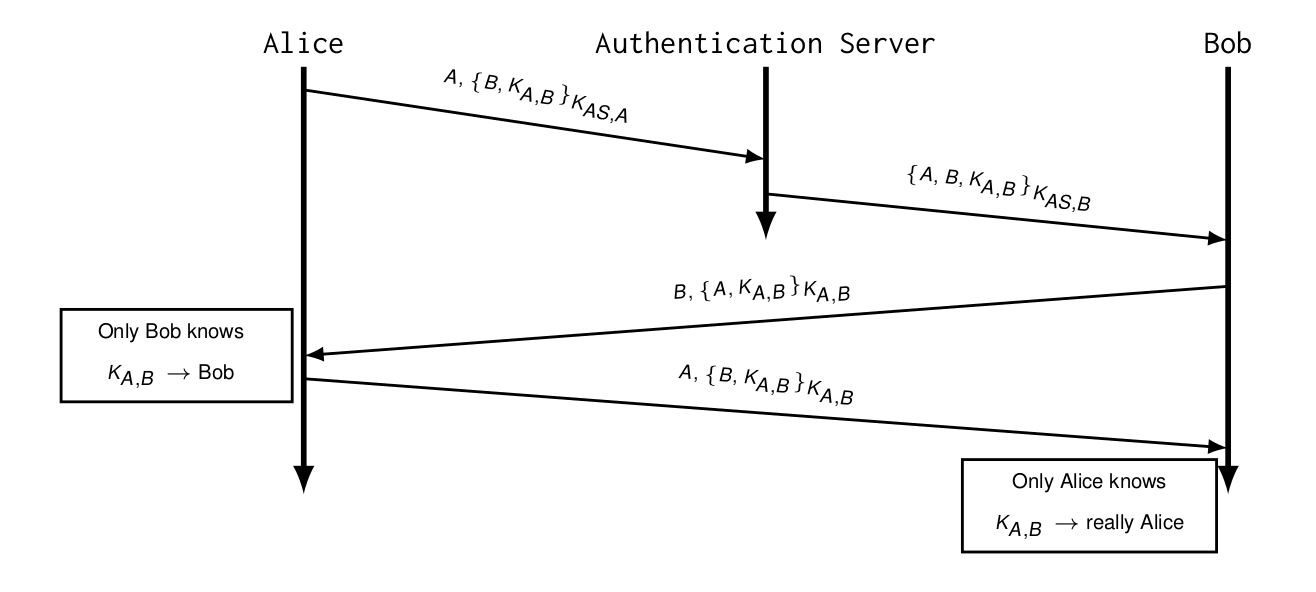
\includegraphics[width=.8\textwidth]{figures/ooppt1.png}
  \caption{Protocol Try 1}\label{fig:ooppt1}
\end{figure}
\newpage

To prevent replay attacks, it is advisable to use fresh nonces for every protocol run.
Figure~\ref{fig:oopp_replay_attack} shows a possible attack and Figure~\ref{fig:ooppt2} an improved protocol.
\begin{figure}[H]
  \centering
  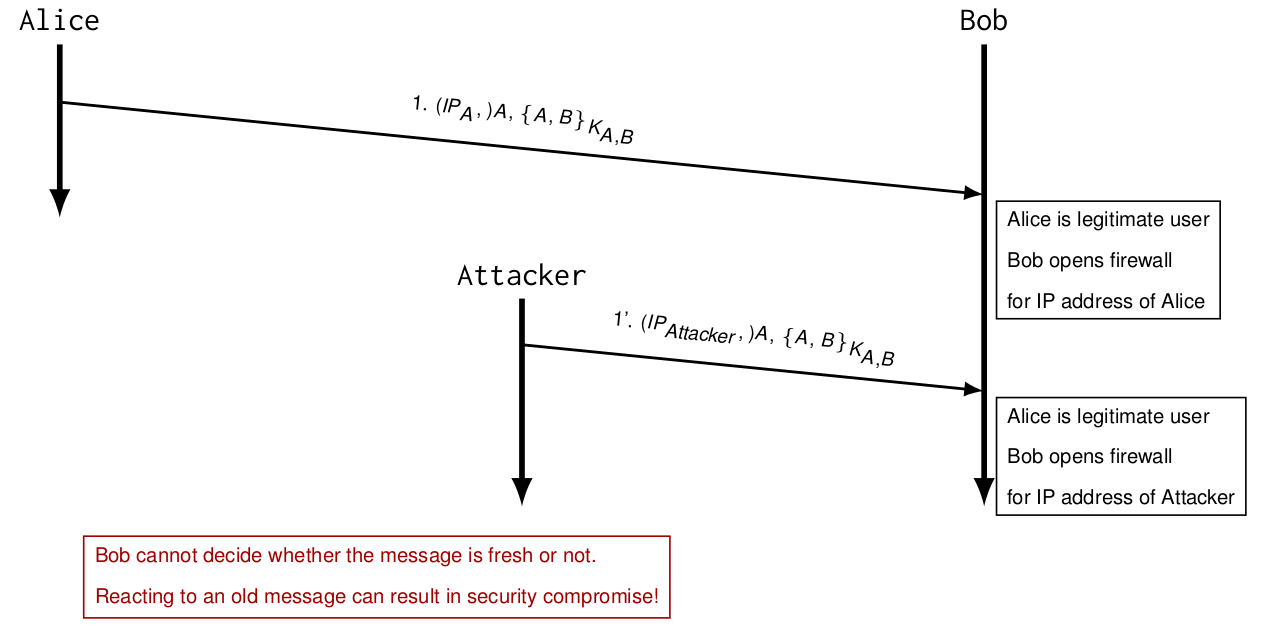
\includegraphics[width=\textwidth]{figures/oopp_replay_attack.png}
  \captionof{figure}{Replay Attack on our Protocol}\label{fig:oopp_replay_attack}
\end{figure}
\begin{figure}[H]
  \centering
  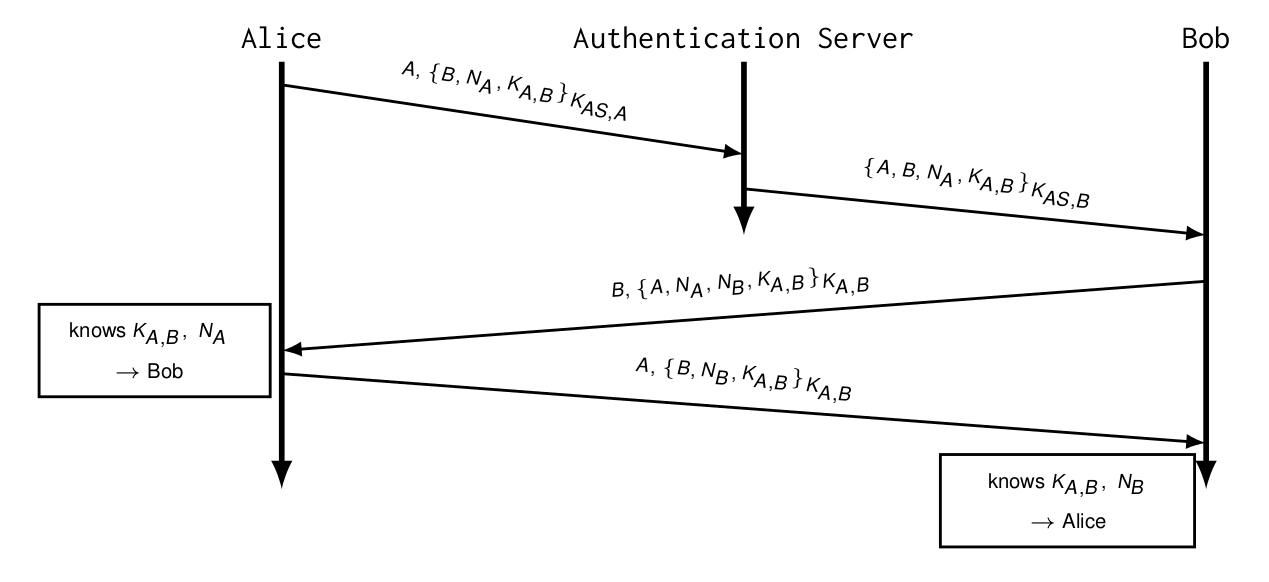
\includegraphics[width=\textwidth]{figures/ooppt2.png}
  \captionof{figure}{Protocol with Nonces}\label{fig:ooppt2}
\end{figure}

Having dealt with that, another problem presents itself: oracle attacks are still possible (c.f.\ Figure~\ref{fig:oopp_oracle_attack}).
\begin{figure}[H]
  \centering
  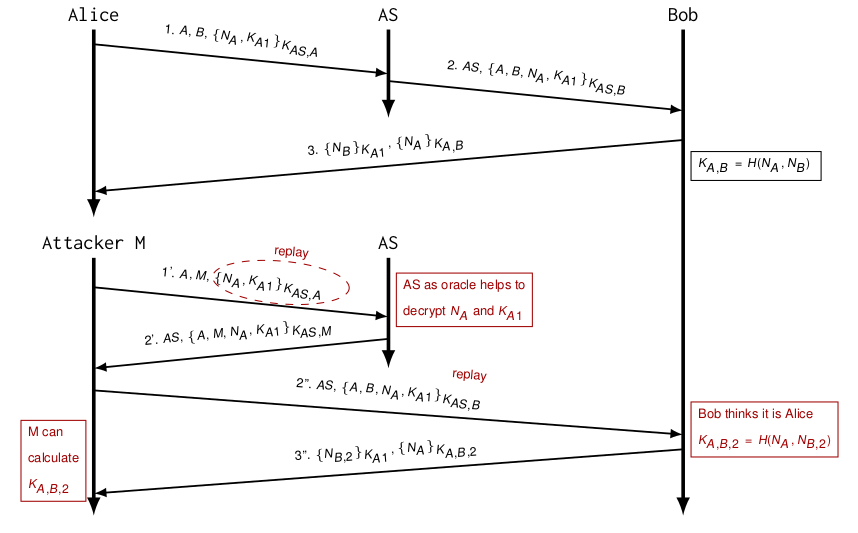
\includegraphics[width=\textwidth]{figures/oopp_oracle_attack.png}
  \caption{Oracle Attack on our Protocol}\label{fig:oopp_oracle_attack}
\end{figure}
\newpage

Now we can add forward secrecy by using Diffie-Hellman as shown in Figure~\ref{fig:ooppt3}.
$DH_B$ is integrity protected because ${A, N_A, N_B}_{K_{A,B}}$ is already encrypted with the key derived from the Diffie-Hellman exchange.
If $DH_B$ is changed by an attacker, Alice cannot decrypt the message anymore.
\begin{figure}[H]
  \centering
  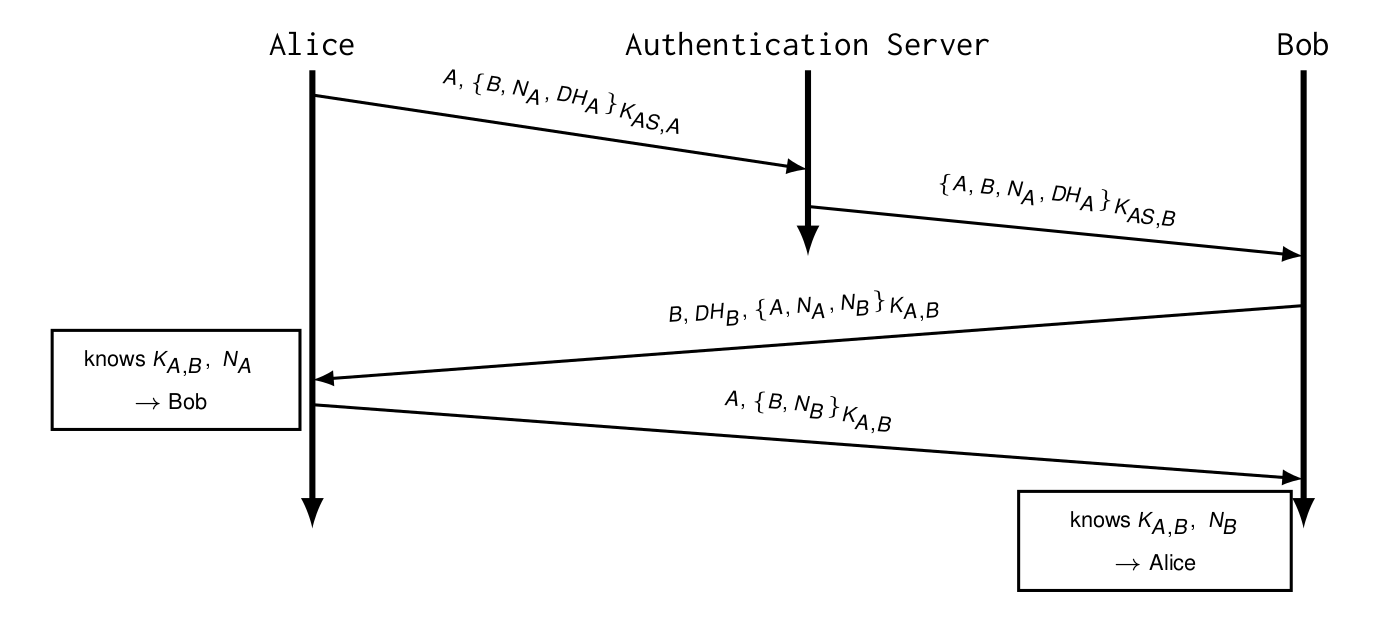
\includegraphics[width=\textwidth]{figures/ooppt3.png}
  \caption{Protocol with Forward Secrecy}\label{fig:ooppt3}
\end{figure}

To improve reliability, we remove the single point of failure, i.e.\ the authentication server, from single protocol runs, 
It might still be used beforehand to provide keys or certificates.
\begin{figure}[H]
  \centering
  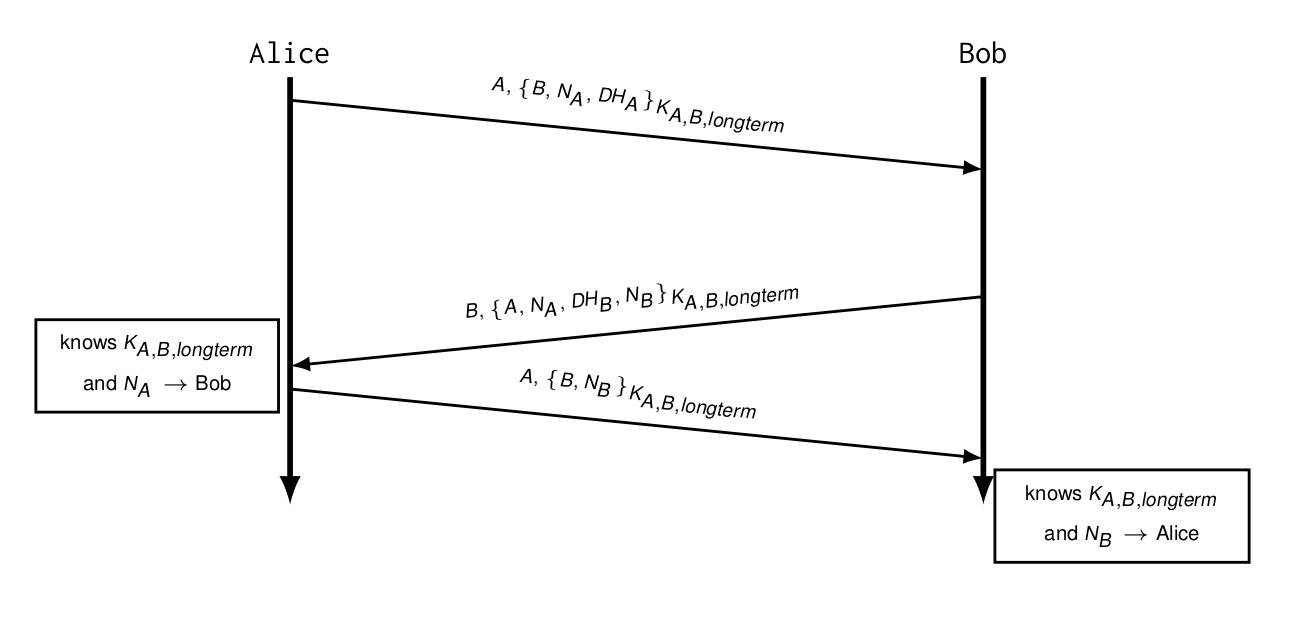
\includegraphics[width=\textwidth]{figures/ooppt4.png}
  \caption{Protocol without Authentication Server}\label{fig:ooppt3}
\end{figure}
\newpage

To simplify key management and authentication, we want to use public key cryptography.
Furthermore we want to include a mechanism that lets Alice and Bob determine which crypto algorithms to use (e.g.\ to stay on the state of the art without changing the protocol).
\begin{figure}[H]
  \centering
  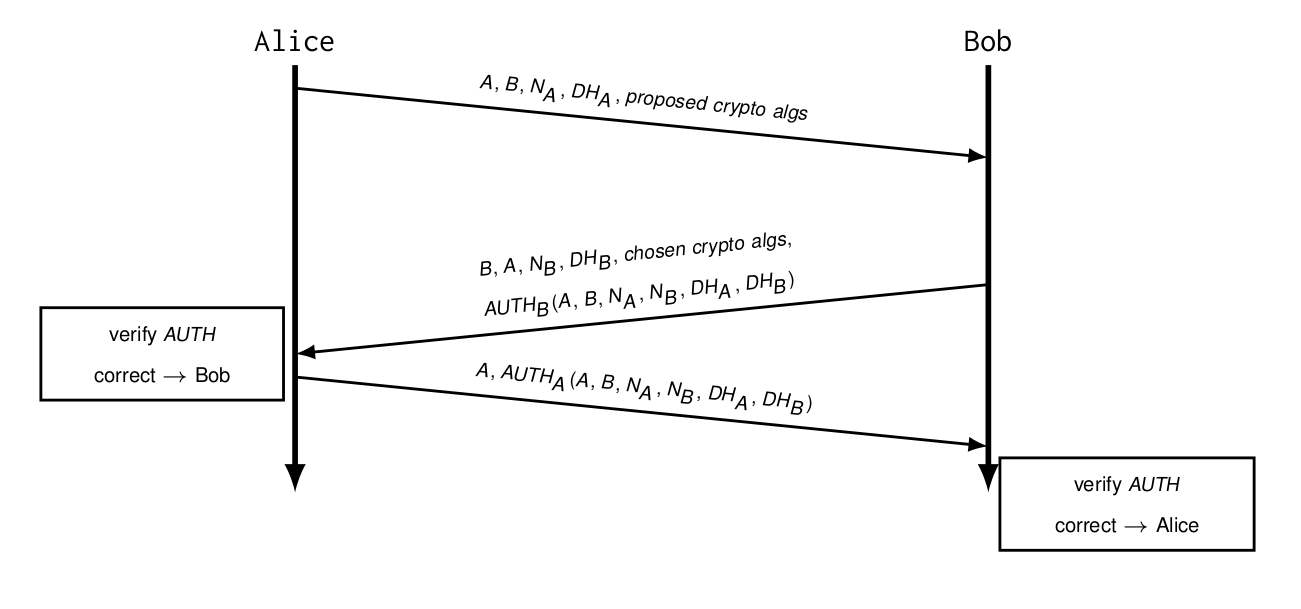
\includegraphics[width=\textwidth]{figures/ooppt5.png}
  \caption{Protocol with Public-key Cryptography and Crypto Algorithm Handshake}\label{fig:ooppt5}
\end{figure}

In case symmetric cryptography is used for AUTH, a replay attack is possible because Alice and Bob authenticate identical messages with the same key in that scenario.
For this reason, we change the authenticated messages.
\begin{figure}[H]
  \centering
  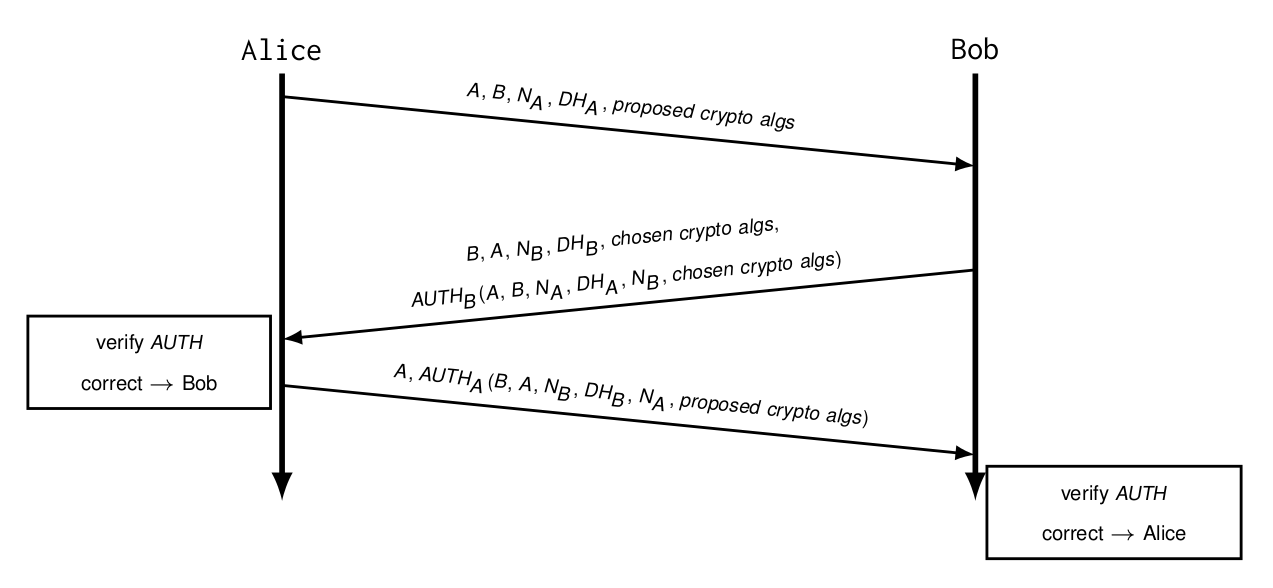
\includegraphics[width=\textwidth]{figures/ooppt6.png}
  \caption{Protocol with different Authenticated Messages}\label{fig:ooppt6}
\end{figure}
\newpage

To decrease complexity, what makes analysis easier and the attack surface smaller, we split the second message into two (request-response pairs).
\begin{figure}[H]
  \centering
  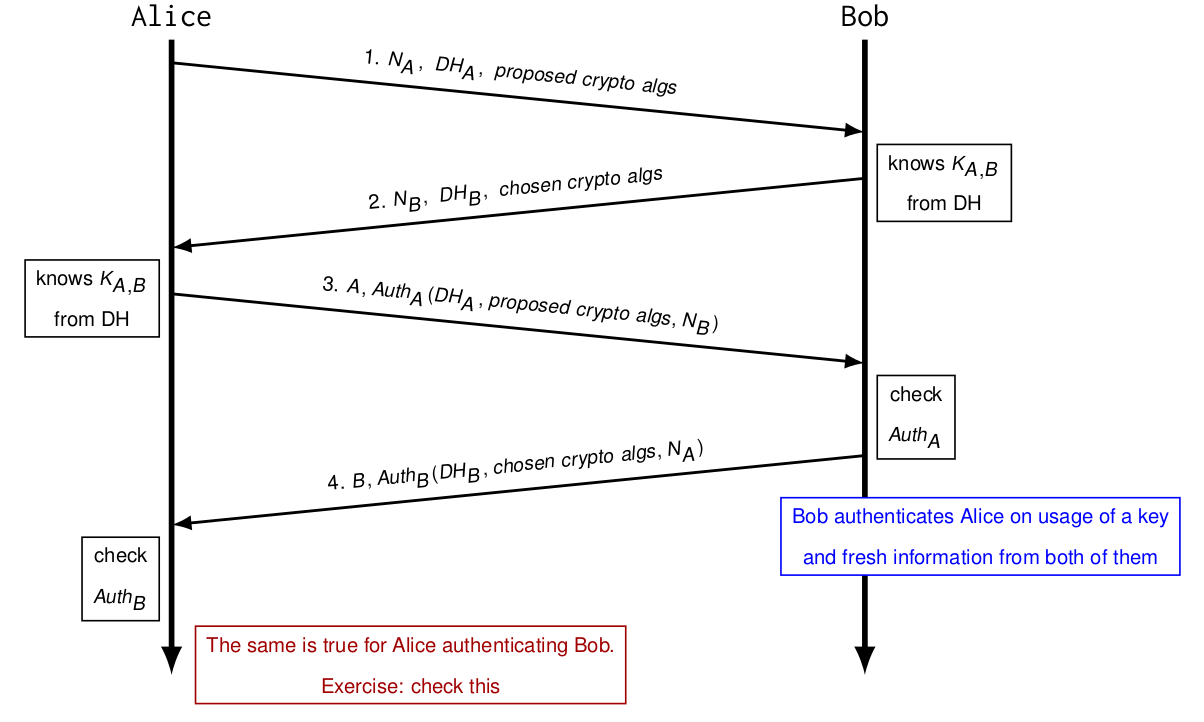
\includegraphics[width=\textwidth]{figures/ooppt7.png}
  \caption{Protocol simplified}\label{fig:ooppt7}
\end{figure}
Messages 1 and 2 are only used for information exchange.
3 and 4 are used for authentication and if any verification fails, communication has to be aborted.

\subsection{Needham Schroeder Protocol (NSP)}
NSP is a protocol for mutual authentication and key establishment over an insecure network.
There is a symmetric key version and a public-key version of it.

\subsubsection{Symmetric Key NSP}
\begin{figure}[H]
\centering
\begin{subfigure}{.5\textwidth}
  \centering
  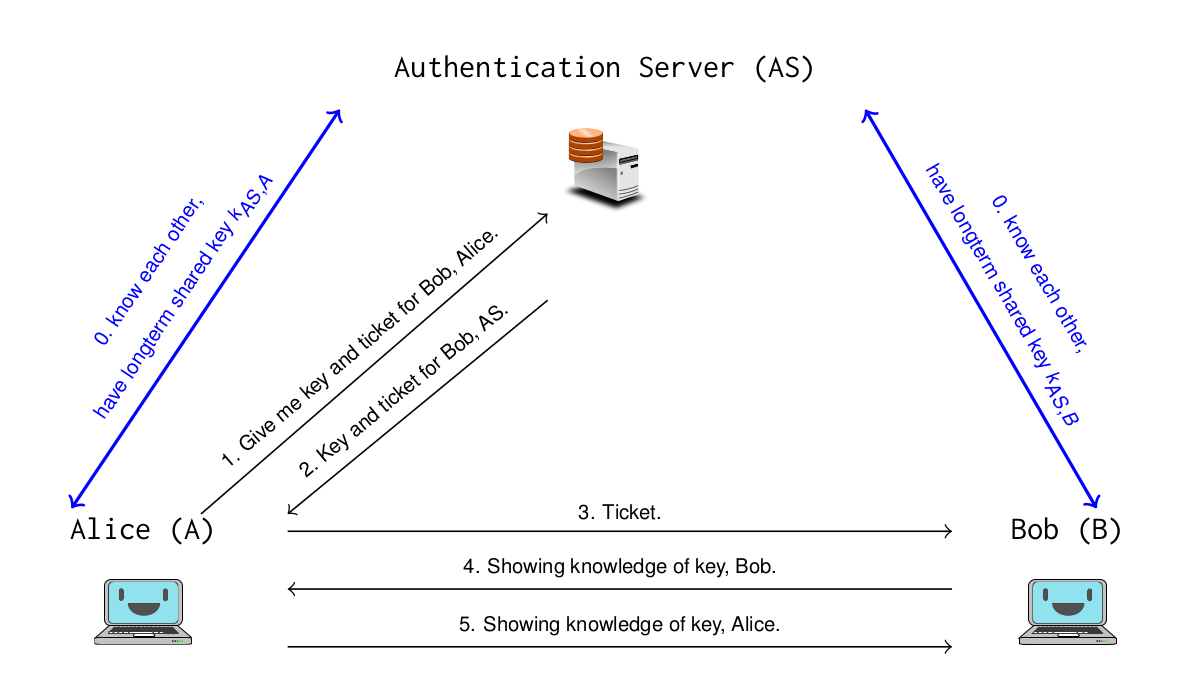
\includegraphics[width=\textwidth]{figures/symmetric_nsp_1.png}
\end{subfigure}%
\begin{subfigure}{.5\textwidth}
  \centering
  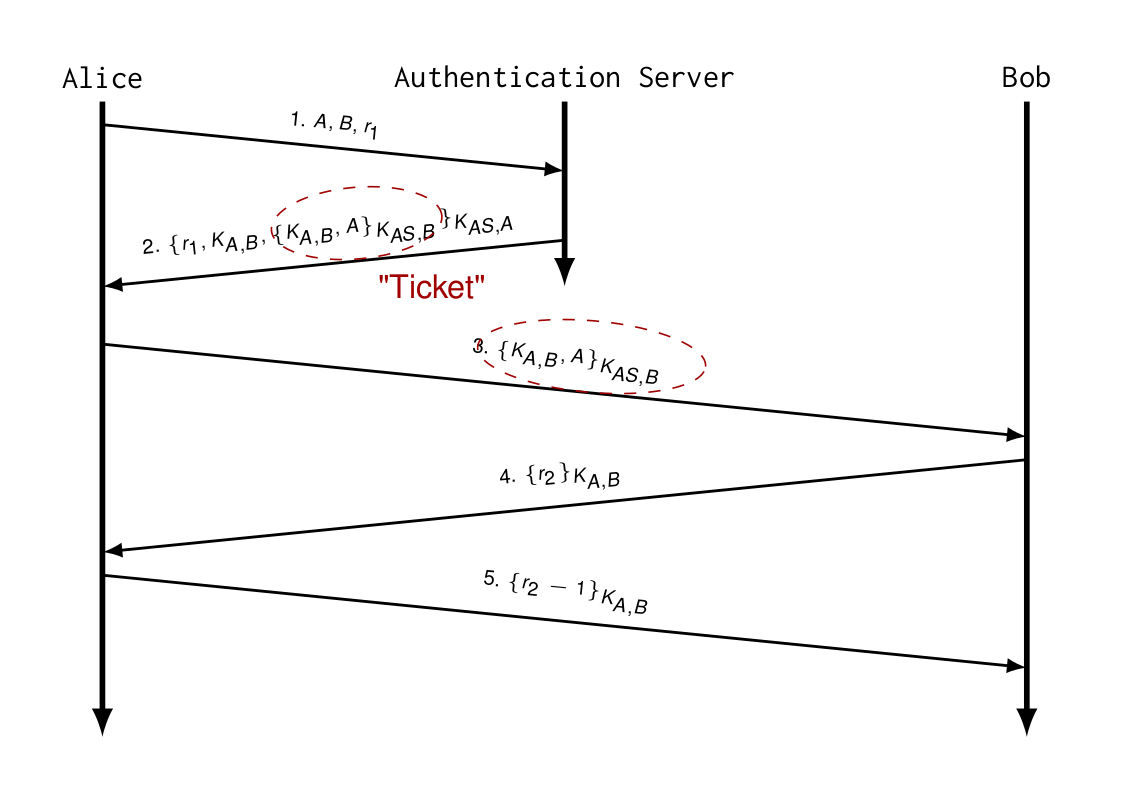
\includegraphics[width=\textwidth]{figures/symmetric_nsp_2.png}
\end{subfigure}
\caption{Symmetric NSP}\label{fig:symmetric_nsp}
\end{figure}
$r_i$ are random values here.
Note here that NSP does not provide forward secrecy.

\subsubsection{Public Key NSP}
\begin{figure}[H]
\centering
\begin{subfigure}{.5\textwidth}
  \centering
  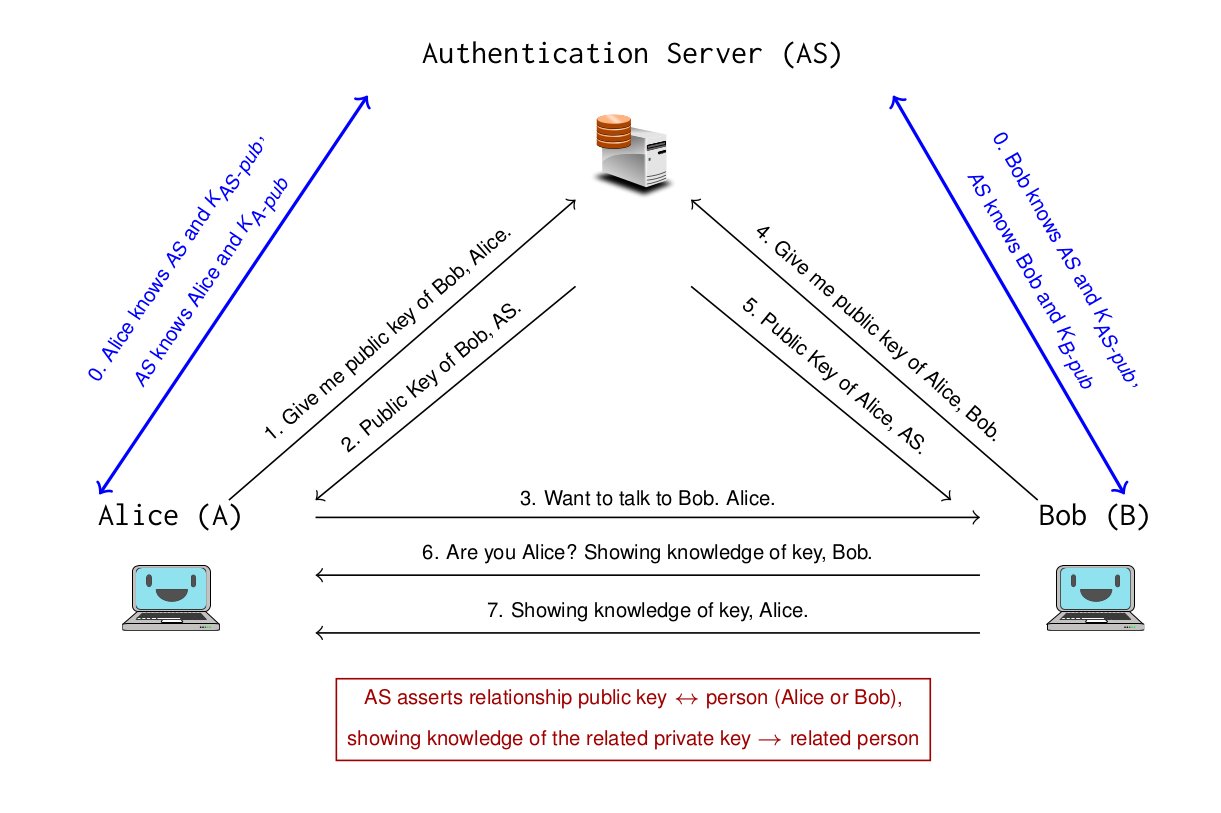
\includegraphics[width=\textwidth]{figures/asymmetric_nsp_1.png}
\end{subfigure}%
\begin{subfigure}{.5\textwidth}
  \centering
  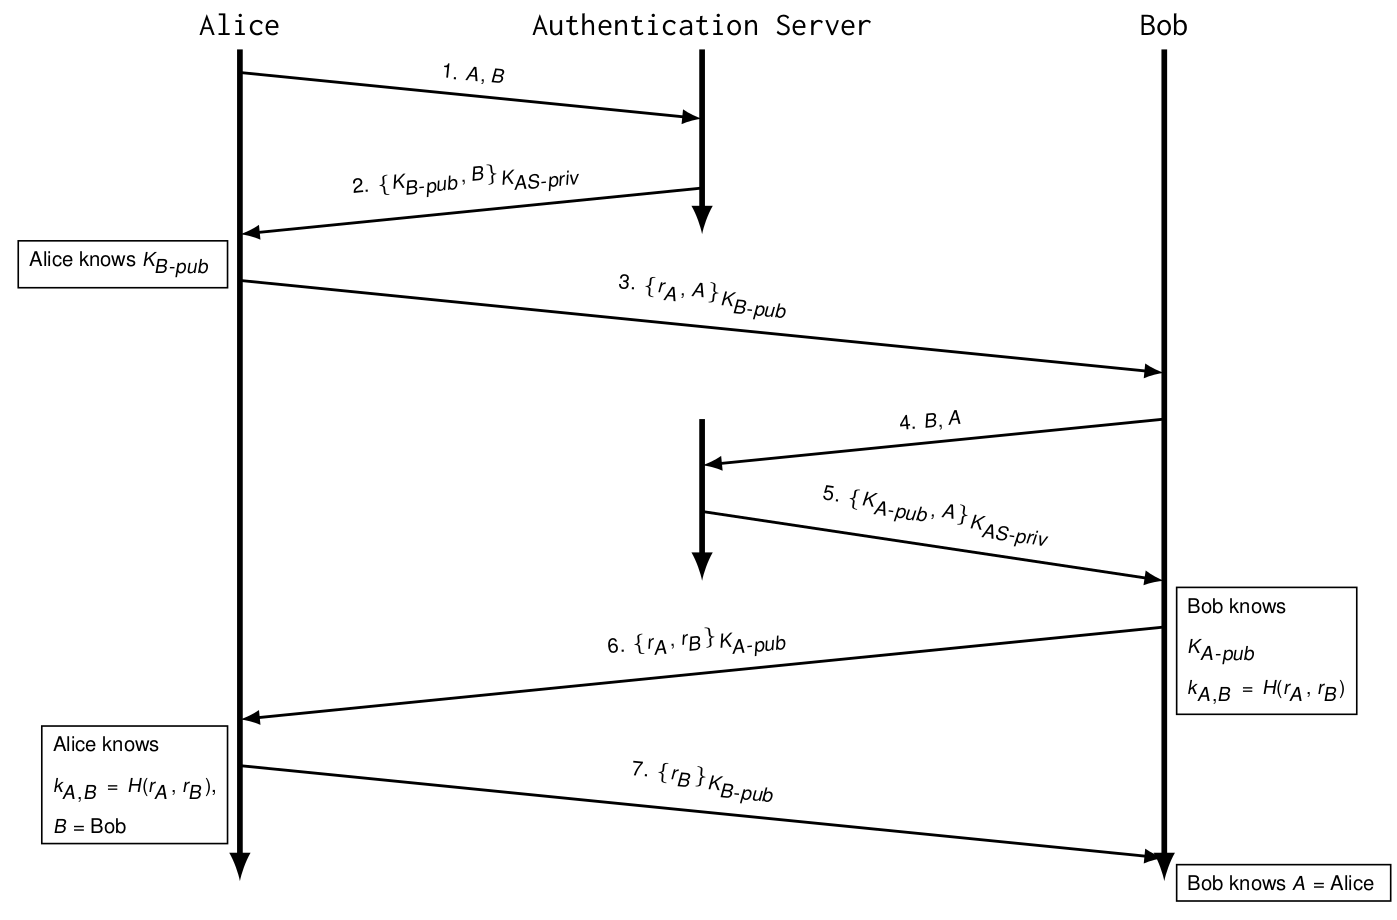
\includegraphics[width=\textwidth]{figures/asymmetric_nsp_2.png}
\end{subfigure}
\caption{Asymmetric NSP}\label{fig:asymmetric_nsp}
\end{figure}
We use $\{\cdot \}$ for encryption and signing here, never mix them up in practice!

\paragraph{Attack on the Public key NSP}
\begin{figure}[H]
  \centering
  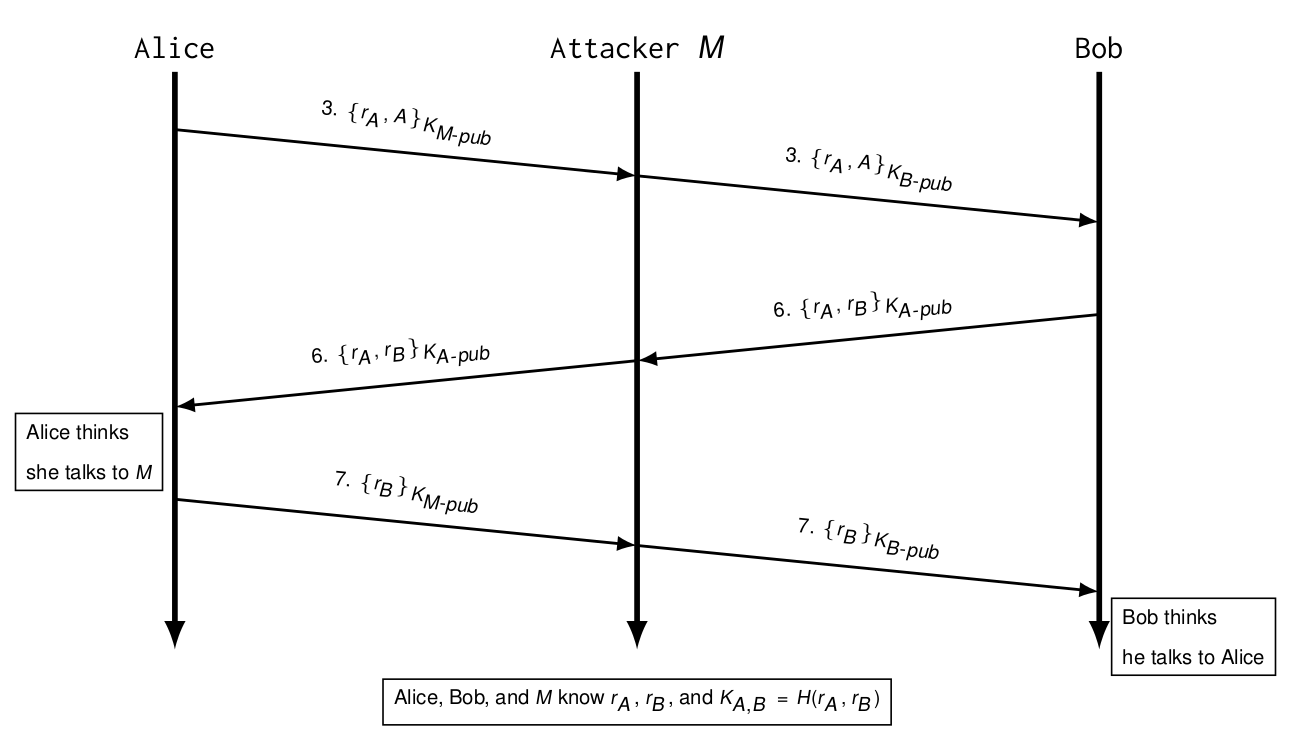
\includegraphics[width=.7\textwidth]{figures/asymmetric_nsp_attack.png}
  \caption{Asymmetric NSP Attack}\label{fig:asymmetric_nsp_attack}
\end{figure}
The idea of the attack is that the attacker M tricks Alice to communicate with him and makes Bob believe, that he talks to Alice.
